\documentclass[conference]{IEEEtran}
\IEEEoverridecommandlockouts

\usepackage{cite}
\usepackage{amsmath,amssymb,amsfonts,amsthm}
\usepackage{algorithm}
\usepackage{algorithmic}
\usepackage{graphicx}
\usepackage{textcomp}
\usepackage{xcolor}
\usepackage{booktabs}
\usepackage{multirow}
\usepackage{array}
\usepackage{url}
\usepackage{hyperref}
\usepackage{tikz}
\usetikzlibrary{arrows.meta,positioning,shapes.geometric,shapes.misc,fit,calc,matrix}

\newtheorem{property}{Property}
\newtheorem{definition}{Definition}

\newcommand{\RACS}{\mathrm{RACS}}
\newcommand{\ERR}{\mathrm{ERR}}
\newcommand{\TFP}{\mathrm{TFP}}
\newcommand{\RP}{\mathrm{RP}}
\newcommand{\ESA}{\mathrm{ESA}}
\newcommand{\JRS}{\mathrm{JRS}}
\newcommand{\Eprev}{E_{\mathrm{prev}}}
\newcommand{\Ecurr}{E_{\mathrm{curr}}}
\newcommand{\Fflag}{F_{\mathrm{flagged}}}

\def\BibTeX{{\rm B\kern-.05em{\sc i\kern-.025em b}\kern-.08em
    T\kern-.1667em\lower.7ex\hbox{E}\kern-.125emX}}

\begin{document}

\title{Regression-Aware Evaluation of Iterative LLM Proof Correction for Optimization and Machine Learning}

\author{
\IEEEauthorblockN{Anonymous Author(s)}
\IEEEauthorblockA{
\textit{Department / Institution}\\
City, Country\\
email@example.com}
}

\maketitle

\begin{abstract}
Large language models can produce plausible long-form mathematical proofs, but their iterative correction behavior remains difficult to evaluate. In optimization and machine learning proofs, a local repair can resolve one missing inequality while introducing a new assumption misuse, algebraic error, or unsupported convergence claim elsewhere. Standard final-verdict evaluation hides this non-monotonic trajectory. This paper develops a methodology for studying iterative proof correction at the level of proof-state transitions. We present a stateful prover--judge pipeline for generating, auditing, and revising LaTeX convergence proofs; a reliability-weighted multi-judge evaluation method based on step-level error-set agreement; and the Regression-Aware Correction Score (RACS), a transition metric that balances error resolution, targeted fix precision, and regression penalization. The proposed framework is designed to occupy the middle ground between coarse LLM-as-judge scoring and full formal verification: it is granular enough to expose correction dynamics while remaining applicable to broad natural-language proof tasks. We further define an ablation protocol for calibrating the RACS weights as correction-incentive parameters. Experimental results, benchmark comparisons, and human/expert validation are intentionally left as dedicated slots to be populated after the final evaluation runs.
\end{abstract}

\begin{IEEEkeywords}
Large Language Models, Mathematical Reasoning, Proof Correction, Agentic AI, LLM-as-Judge, Optimization, Regression-Aware Evaluation
\end{IEEEkeywords}

\section{Introduction}
Large language models (LLMs) are increasingly capable of producing mathematical text that resembles expert derivations. Yet in rigorous optimization and machine learning (OML), proof quality depends on more than fluent theorem statements. A valid convergence proof requires a chain of mutually dependent assumptions, inequalities, expectation manipulations, operator identities, and rate extractions. A single invalid inequality can invalidate all downstream reasoning.

One natural response is iterative correction: generate a proof, critique it, revise it, and repeat. However, this process is not monotonic. A model may repair a flagged smoothness argument while damaging a previously correct stochastic expectation step; it may add a missing lemma while silently strengthening an assumption; or it may satisfy the wording of feedback without restoring the global convergence argument. Final pass/fail evaluation cannot distinguish a stable correction from a fragile trajectory that happens to end well.

This paper argues that iterative LLM proof correction should be evaluated as a proof-state trajectory rather than a single final artifact. Our setting focuses on informal but structured LaTeX convergence proofs, where full translation into proof assistants such as Lean or Coq may be impractical for every algorithmic variant, but where unstructured natural-language judging is too coarse to support scientific measurement.

We make the following methodological contributions:
\begin{itemize}
    \item We formalize iterative proof correction as transitions between proof states and evaluator error sets.
    \item We present a prover--judge pipeline that uses step-level annotations and structured evaluator outputs to make proof errors auditable.
    \item We define a multi-judge consensus method in which evaluator reliability is estimated using step-level error-set agreement and score deviation.
    \item We introduce the Regression-Aware Correction Score (RACS), a metric for evaluating whether a correction transition fixed known errors, followed targeted feedback, and avoided new regressions.
    \item We specify an ablation protocol that treats RACS weights as correction-incentive parameters rather than arbitrary constants.
\end{itemize}

The remainder of this paper is structured as a methodology-first research article. Sections~\ref{sec:problem}--\ref{sec:ablation} can be finalized before empirical results are available. Sections~\ref{sec:experiments}--\ref{sec:results} are designed to reserve space for benchmark results, ablation plots, and expert validation once the final experiments are complete.

\section{Related Work}
LLM mathematical reasoning has been studied through chain-of-thought prompting, self-correction, and tool-augmented proof generation. Systems such as Minerva~\cite{lewkowycz2022minerva} demonstrate the potential of language models for mathematical problem solving, while methods such as Self-Refine~\cite{madaan2023selfrefine} and Reflexion~\cite{shinn2023reflexion} show that iterative feedback can improve model outputs. In parallel, formal theorem proving systems, including Lean~\cite{demoura2015lean}, provide strong correctness guarantees but require formalized statements and machine-checkable proof scripts.

LLM-as-judge evaluation has also become common for open-ended outputs~\cite{zheng2023judging}. However, proof correction differs from general response grading because errors are localized, structured, and often coupled across steps. A judge must identify not only whether a proof is acceptable, but which proof steps contain missing derivations, unsupported claims, operator mistakes, or assumption violations.

This work sits between informal judging and formal verification. It does not claim theorem-prover-level guarantees. Instead, it proposes a structured trajectory-evaluation methodology that can measure correction quality in natural-language mathematical proofs while preserving enough granularity to audit the dynamics of repair.

\section{Problem Definition}
\label{sec:problem}

\subsection{Proof-State Trajectories}
Let $\mathcal{P}_0$ denote the initial proof generated by an LLM prover. At correction iteration $i$, the system holds a proof state $\mathcal{P}_i$. A judge or judge ensemble evaluates $\mathcal{P}_i$ and returns a structured error set $E_i$ and a flagged-step set $F_i$.

We represent the iterative process as:
\begin{equation}
    \mathcal{P}_0 \xrightarrow[]{E_0,F_0}
    \mathcal{P}_1 \xrightarrow[]{E_1,F_1}
    \cdots
    \mathcal{P}_T.
\end{equation}
The central evaluation object is the transition $\mathcal{P}_i \rightarrow \mathcal{P}_{i+1}$, not merely the final proof $\mathcal{P}_T$.

\subsection{Step-Level Error Sets}
Each proof is required to annotate non-trivial derivation steps using explicit step markers such as \texttt{[Step 7]}. Evaluators return error sets over these step identifiers. In the implementation, the primary error categories are:
\begin{itemize}
    \item hallucinated or unsupported claims,
    \item missing derivation steps,
    \item operator, algebraic, or analytic manipulation errors,
    \item assumption misuse or assumption violations.
\end{itemize}

The union of these per-category sets gives a step-level error set:
\begin{equation}
    E_i =
    E_i^{\mathrm{HA}}
    \cup E_i^{\mathrm{MS}}
    \cup E_i^{\mathrm{OP}}
    \cup E_i^{\mathrm{AV}}.
\end{equation}

\subsection{Correction Transition Types}
For consecutive error sets $\Eprev$ and $\Ecurr$, a correction transition decomposes into:
\begin{align}
    \mathrm{Fixed} &= \Eprev \setminus \Ecurr, \\
    \mathrm{Persistent} &= \Eprev \cap \Ecurr, \\
    \mathrm{Regressed} &= \Ecurr \setminus \Eprev.
\end{align}
A transition is \emph{mixed} if it fixes at least one previous error while introducing at least one new error:
\begin{equation}
    (\Eprev \setminus \Ecurr) \neq \emptyset
    \quad \wedge \quad
    (\Ecurr \setminus \Eprev) \neq \emptyset.
\end{equation}
Mixed transitions are central to this paper because they expose the non-monotonicity of LLM proof repair.

\begin{figure}[t]
\centering
\resizebox{\columnwidth}{!}{%
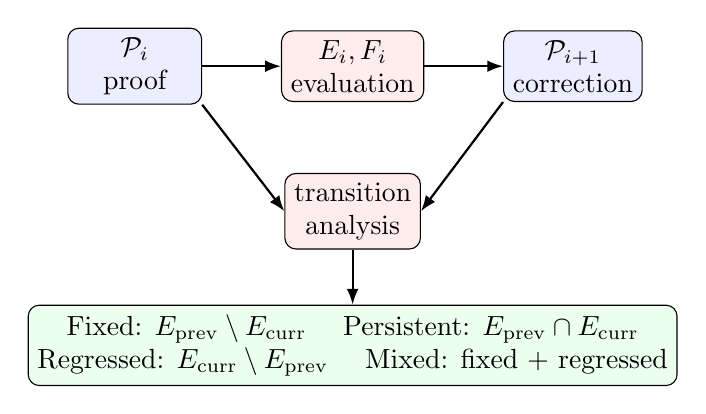
\begin{tikzpicture}[
    node distance=7mm,
    proof/.style={draw, rounded corners, align=center, minimum width=1.7cm, minimum height=0.65cm, fill=blue!7},
    err/.style={draw, rounded corners, align=center, minimum width=1.7cm, minimum height=0.65cm, fill=red!7},
    arrow/.style={-{Latex[length=2mm]}, thick}
]
\node[proof] (p0) {$\mathcal{P}_i$\\proof};
\node[err, right=10mm of p0] (e0) {$E_i,F_i$\\evaluation};
\node[proof, right=10mm of e0] (p1) {$\mathcal{P}_{i+1}$\\correction};
\node[err, below=9mm of e0] (delta) {transition\\analysis};
\draw[arrow] (p0) -- (e0);
\draw[arrow] (e0) -- (p1);
\draw[arrow] (p0.south east) -- (delta.west);
\draw[arrow] (p1.south west) -- (delta.east);
\node[draw, rounded corners, fill=green!7, below=7mm of delta, align=center, minimum width=5.5cm] (sets)
{Fixed: $\Eprev\setminus\Ecurr$ \quad Persistent: $\Eprev\cap\Ecurr$\\
Regressed: $\Ecurr\setminus\Eprev$ \quad Mixed: fixed $+$ regressed};
\draw[arrow] (delta) -- (sets);
\end{tikzpicture}
}
\caption{A correction transition is evaluated by comparing error sets before and after revision.}
\label{fig:transition}
\end{figure}

\section{System Architecture}
\label{sec:architecture}

\subsection{Overview}
The implementation uses a stateful LangGraph workflow with two main roles: a prover and an evaluator. The prover constructs or revises a convergence proof. The evaluator audits the proof and emits structured feedback. If the proof does not pass, the feedback is routed back to the prover for correction.

\begin{figure*}[t]
\centering
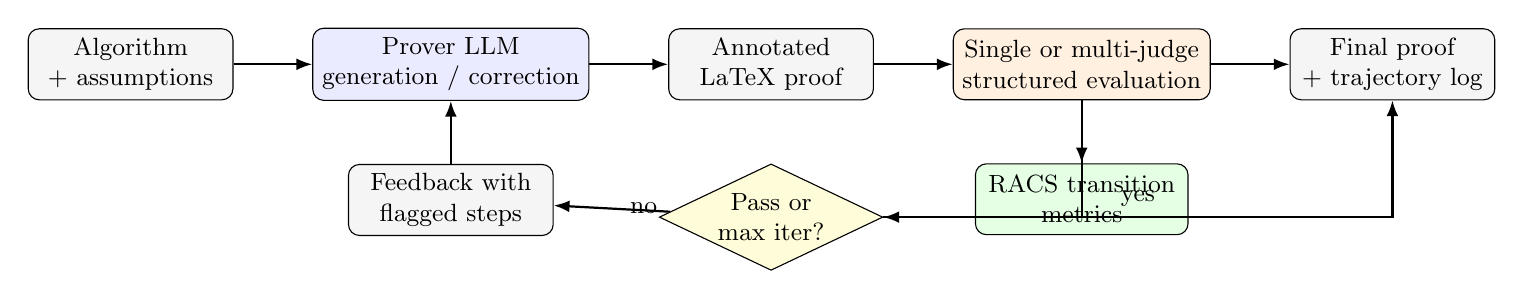
\begin{tikzpicture}[
    font=\small,
    node distance=8mm and 10mm,
    block/.style={draw, rounded corners, align=center, minimum width=2.6cm, minimum height=0.85cm, fill=gray!8},
    agent/.style={draw, rounded corners, align=center, minimum width=2.7cm, minimum height=0.9cm, fill=blue!8},
    judge/.style={draw, rounded corners, align=center, minimum width=2.7cm, minimum height=0.9cm, fill=orange!12},
    metric/.style={draw, rounded corners, align=center, minimum width=2.7cm, minimum height=0.9cm, fill=green!10},
    decision/.style={draw, diamond, aspect=2.1, align=center, inner sep=1pt, fill=yellow!15},
    arrow/.style={-{Latex[length=2mm]}, thick}
]
\node[block] (input) {Algorithm\\+ assumptions};
\node[agent, right=of input] (prover) {Prover LLM\\generation / correction};
\node[block, right=of prover] (proof) {Annotated\\LaTeX proof};
\node[judge, right=of proof] (eval) {Single or multi-judge\\structured evaluation};
\node[metric, below=of eval] (racs) {RACS transition\\metrics};
\node[decision, below=of proof] (pass) {Pass or\\max iter?};
\node[block, below=of prover] (feedback) {Feedback with\\flagged steps};
\node[block, right=of eval] (output) {Final proof\\+ trajectory log};

\draw[arrow] (input) -- (prover);
\draw[arrow] (prover) -- (proof);
\draw[arrow] (proof) -- (eval);
\draw[arrow] (eval) -- (racs);
\draw[arrow] (eval) |- (pass);
\draw[arrow] (pass) -- node[right, xshift=1mm] {no} (feedback);
\draw[arrow] (feedback) -- (prover);
\draw[arrow] (pass.east) -| node[above, pos=0.25] {yes} (output.south);
\draw[arrow] (eval) -- (output);
\end{tikzpicture}
\caption{Stateful proof-correction pipeline. The prover is constructive, while evaluation is conservative, structured, and near-deterministic.}
\label{fig:pipeline}
\end{figure*}

\subsection{Design Rationale}
\textbf{Role separation.} Proof generation and proof reviewing are different tasks. The prover is allowed to explore proof paths, while the judge is constrained to produce structured, low-temperature critiques. This separation reduces self-reinforcement of the prover's own mistakes and produces auditable measurement signals.

\textbf{Step annotations.} Requiring explicit proof-step identifiers turns vague mathematical feedback into set-valued objects. These objects support targeted correction, judge agreement computation, and regression detection.

\textbf{Phase-aware sampling.} The system uses higher stochasticity for initial proof construction, lower stochasticity for correction, and near-deterministic settings for evaluation. This reflects the difference between creative proof search and stable proof auditing.

\section{Multi-Judge Consensus and JRS}
\label{sec:jrs}

\subsection{Independent Structured Evaluators}
In multi-judge mode, several evaluator models independently review the same proof. Each judge returns a JSON object containing an overall verdict, scalar scores, detailed feedback, per-category step-level error sets, and flagged steps for the next correction.

\subsection{Error-Set Agreement}
For judges $a$ and $b$, let $E^{(a)}$ and $E^{(b)}$ be their step-level error sets. Error Set Agreement (ESA) is defined as Jaccard similarity:
\begin{equation}
    \ESA(a,b) =
    \frac{|E^{(a)} \cap E^{(b)}|}
         {|E^{(a)} \cup E^{(b)}|},
\end{equation}
with $\ESA(a,b)=1$ when both judges report no errors. The mean agreement of judge $j$ with the rest of the ensemble is denoted $\ESA_j$.

\subsection{Judge Reliability Score}
Each judge also receives a scalar quality score, such as a mean of completeness and assumption-use scores. Let $z_j$ be the standardized deviation of judge $j$'s score from the ensemble mean. The Judge Reliability Score is:
\begin{equation}
    \JRS_j = \alpha \ESA_j - \beta |z_j|.
\end{equation}
The first term rewards agreement on concrete error localization. The second term penalizes score outliers. JRS is not a formal certificate of correctness; it is a consensus reliability heuristic that makes evaluator influence auditable.

\begin{figure}[t]
\centering
\resizebox{\columnwidth}{!}{%
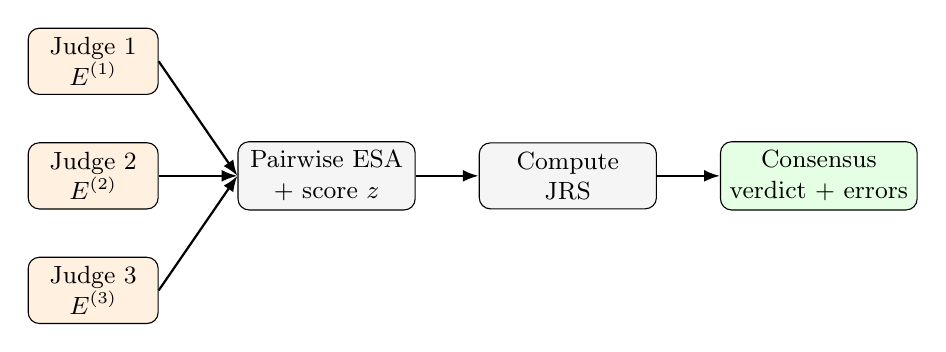
\begin{tikzpicture}[
    font=\small,
    node distance=6mm,
    judge/.style={draw, rounded corners, align=center, minimum width=1.65cm, minimum height=0.7cm, fill=orange!12},
    proc/.style={draw, rounded corners, align=center, minimum width=2.25cm, minimum height=0.75cm, fill=gray!8},
    outbox/.style={draw, rounded corners, align=center, minimum width=2.4cm, minimum height=0.75cm, fill=green!10},
    arrow/.style={-{Latex[length=2mm]}, thick}
]
\node[judge] (j1) {Judge 1\\$E^{(1)}$};
\node[judge, below=of j1] (j2) {Judge 2\\$E^{(2)}$};
\node[judge, below=of j2] (j3) {Judge 3\\$E^{(3)}$};
\node[proc, right=10mm of j2] (esa) {Pairwise ESA\\+ score $z$};
\node[proc, right=8mm of esa] (jrs) {Compute\\JRS};
\node[outbox, right=8mm of jrs] (cons) {Consensus\\verdict + errors};

\draw[arrow] (j1.east) -- (esa.west);
\draw[arrow] (j2.east) -- (esa.west);
\draw[arrow] (j3.east) -- (esa.west);
\draw[arrow] (esa) -- (jrs);
\draw[arrow] (jrs) -- (cons);
\end{tikzpicture}
}
\caption{Multi-judge consensus converts independent structured reviews into a reliability-weighted evaluation.}
\label{fig:jrs}
\end{figure}

\subsection{Consensus Output}
The consensus stage aggregates both verdict and error sets. In the implementation, verdicts are mapped to ordinal scores and aggregated with reliability-aware weights. Per-type error sets are majority-merged to avoid allowing a single noisy judge to dominate official error localization. Flagged steps are union-merged so the prover receives inclusive repair guidance.

\section{Regression-Aware Correction Score}
\label{sec:racs}

\subsection{Metric Definition}
Let $\Eprev$ and $\Ecurr$ be the previous and current error sets, and let $\Fflag$ be the set of steps explicitly flagged for repair. RACS decomposes a correction transition into three components.

\begin{align}
    \ERR &= \frac{|\Eprev \setminus \Ecurr|}{|\Eprev|}, \\
    \TFP &= \frac{|\Fflag \setminus \Ecurr|}{|\Fflag|}, \\
    \RP &= \min\left(1,\frac{|\Ecurr \setminus \Eprev|}{\max(1,|\Eprev|)}\right).
\end{align}
When $\Eprev=\emptyset$, $\ERR$ is defined as $1$ for delta-based transitions. When $\Fflag=\emptyset$, $\TFP$ is defined as $1$.

The composite score is:
\begin{equation}
    \RACS_{\mathrm{raw}}
    =
    (w_{\mathrm{err}}\ERR + w_{\mathrm{tfp}}\TFP)
    (1 - w_{\mathrm{rp}}\RP),
\end{equation}
with $w_{\mathrm{err}}+w_{\mathrm{tfp}}=1$. The final metric is clipped to the unit interval:
\begin{equation}
    \RACS = \min(1,\max(0,\RACS_{\mathrm{raw}})).
\end{equation}

\subsection{Interpretation}
RACS evaluates correction behavior, not generic model intelligence. It measures whether a model:
\begin{itemize}
    \item repairs previously identified mathematical errors,
    \item follows targeted feedback from evaluators,
    \item avoids regressions in previously stable proof regions,
    \item uses critique to improve local and global proof structure,
    \item removes or justifies hallucinated mathematical claims.
\end{itemize}
It is therefore appropriate for guided proof-repair settings, but not intended as a stand-alone score for one-shot proof generation.

\subsection{Properties}
\begin{property}[Boundedness]
$0 \le \RACS \le 1$.
\end{property}

\begin{property}[Perfect Correction Optimality]
If all previous errors are fixed, all flagged steps are resolved, and no new errors are introduced, then $\RACS=1$.
\end{property}

\begin{property}[Regression Monotonicity]
Holding $\ERR$ and $\TFP$ fixed, increasing $\RP$ weakly decreases $\RACS$.
\end{property}

\begin{property}[Mixed-Transition Sensitivity]
When a correction both fixes old errors and introduces new ones, RACS assigns an intermediate transition score rather than collapsing the trajectory into a binary label.
\end{property}

\begin{figure}[t]
\centering
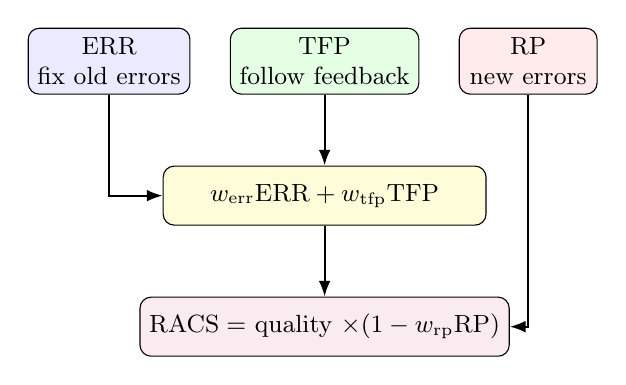
\begin{tikzpicture}[
    font=\small,
    box/.style={draw, rounded corners, align=center, minimum width=1.75cm, minimum height=0.75cm},
    arrow/.style={-{Latex[length=2mm]}, thick}
]
\node[box, fill=blue!8] (err) {ERR\\fix old errors};
\node[box, fill=green!10, right=5mm of err] (tfp) {TFP\\follow feedback};
\node[box, fill=red!8, right=5mm of tfp] (rp) {RP\\new errors};
\node[box, fill=yellow!15, below=9mm of tfp, minimum width=4.1cm] (quality) {$w_{\rm err}\ERR+w_{\rm tfp}\TFP$};
\node[box, fill=purple!8, below=9mm of quality, minimum width=4.1cm] (racs) {$\RACS =$ quality $\times (1-w_{\rm rp}\RP)$};
\draw[arrow] (err) |- (quality);
\draw[arrow] (tfp) -- (quality);
\draw[arrow] (rp) |- (racs);
\draw[arrow] (quality) -- (racs);
\end{tikzpicture}
\caption{RACS rewards resolved and targeted fixes while applying a multiplicative penalty for regressions.}
\label{fig:racs}
\end{figure}

\section{Weight Calibration by Ablation}
\label{sec:ablation}

The RACS weights encode correction incentives. Rather than choosing them purely by intuition, the paper treats them as calibration parameters to be studied through ablation.

\begin{table}[t]
\caption{Correction incentive philosophies encoded by RACS weights.}
\centering
\footnotesize
\begin{tabular}{p{0.18\linewidth}p{0.25\linewidth}p{0.42\linewidth}}
\toprule
\textbf{Emphasis} & \textbf{Dominant incentive} & \textbf{Interpretation} \\
\midrule
High $w_{\rm err}$ & Aggressive error resolution & Prioritize clearing known errors, even if revision is broad. \\
High $w_{\rm tfp}$ & Targeted judge compliance & Prioritize fixing exactly what evaluators flagged. \\
High $w_{\rm rp}$ & Conservative refinement & Prioritize avoiding new errors and preserving stable proof regions. \\
\bottomrule
\end{tabular}
\label{tab:incentives}
\end{table}

\subsection{Ablation Protocol}
The planned calibration protocol is:
\begin{enumerate}
    \item Define a grid over $w_{\rm err}$ and $w_{\rm rp}$.
    \item Set $w_{\rm tfp}=1-w_{\rm err}$.
    \item Run the same proof tasks under each weight configuration.
    \item Compare RACS values against an external quality target.
    \item Select a weight region that balances alignment, interpretability, and trajectory stability.
\end{enumerate}

Possible external targets include expert proof-quality ratings, reviewer rubric scores, final structured judge verdicts, or manually labeled correction outcomes. If the target is judge-derived, the paper should describe it as a judge-verdict proxy rather than human judgment.

\begin{figure}[t]
\centering
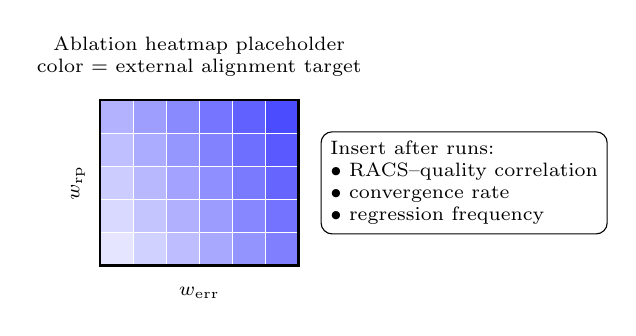
\begin{tikzpicture}[font=\scriptsize]
    \def\cell{0.42}
    \foreach \x in {0,...,5} {
        \foreach \y in {0,...,4} {
            \pgfmathsetmacro{\shade}{10+8*\x+5*\y}
            \fill[blue!\shade] (\x*\cell,\y*\cell) rectangle ++(\cell,\cell);
            \draw[white, line width=0.2pt] (\x*\cell,\y*\cell) rectangle ++(\cell,\cell);
        }
    }
    \draw[thick] (0,0) rectangle (6*\cell,5*\cell);
    \node[below] at (3*\cell,-0.15) {$w_{\rm err}$};
    \node[rotate=90] at (-0.28,2.5*\cell) {$w_{\rm rp}$};
    \node[align=center, above] at (3*\cell,5*\cell+0.18) {Ablation heatmap placeholder\\color = external alignment target};
    \node[draw, rounded corners, fill=white, align=left, anchor=west] at (2.8,1.05)
    {Insert after runs:\\
    $\bullet$ RACS--quality correlation\\
    $\bullet$ convergence rate\\
    $\bullet$ regression frequency};
\end{tikzpicture}
\caption{Planned RACS weight-sensitivity visualization. The final paper should replace this schematic with the empirical ablation heatmap.}
\label{fig:ablation_heatmap}
\end{figure}

\section{Experimental Protocol}
\label{sec:experiments}

\subsection{Task Suite}
The benchmark suite should consist of OML convergence-proof tasks spanning several algorithm families and assumption regimes. Each row should include an algorithm description, assumptions, and preferably a reference proof technique or source family. The final manuscript should report:
\begin{itemize}
    \item number of tasks,
    \item algorithm families,
    \item assumption categories,
    \item model/provider configuration,
    \item maximum correction iterations,
    \item judge ensemble composition,
    \item total cost and latency.
\end{itemize}

\subsection{Baselines}
The following baselines should be included or explicitly marked as future work:
\begin{enumerate}
    \item \textbf{Single-pass prover:} one proof generation, no correction loop.
    \item \textbf{Self-correction without external judge:} the prover critiques and revises itself.
    \item \textbf{Single-judge correction:} one structured evaluator guides correction.
    \item \textbf{Multi-judge majority vote:} ensemble evaluation without JRS weighting.
    \item \textbf{RACS without regression penalty:} ablation removing the distinctive non-monotonicity term.
    \item \textbf{Final-verdict-only scoring:} comparison against static end-state evaluation.
\end{enumerate}

\subsection{Evaluation Axes}
The final results should avoid collapsing all behavior into a single score. Recommended axes are:
\begin{itemize}
    \item final proof verdict,
    \item correction quality via RACS,
    \item number of iterations,
    \item regression frequency,
    \item mixed-transition frequency,
    \item judge agreement and JRS distribution,
    \item cost and latency,
    \item expert or rubric alignment.
\end{itemize}

\begin{table}[t]
\caption{Result slots to be filled after final benchmark runs.}
\centering
\begin{tabular}{p{0.33\linewidth}p{0.52\linewidth}}
\toprule
\textbf{Section} & \textbf{Required content} \\
\midrule
Main benchmark & pass rate, final score, iteration count, cost \\
RACS trajectory & mean/median RACS across correction rounds \\
Ablation & weight heatmap, selected weight rationale \\
Multi-judge & JRS distribution, agreement, outlier rate \\
Failure analysis & representative mixed transitions and judge failures \\
\bottomrule
\end{tabular}
\label{tab:result_slots}
\end{table}

\section{Results and Benchmark Placeholders}
\label{sec:results}

\subsection{Overall Proof Quality}
\noindent\textbf{To be filled after experiments.} Report single-pass versus iterative correction quality, with confidence intervals where appropriate. Avoid claiming improvement unless supported by paired statistical tests.

\subsection{RACS Trajectory Analysis}
\noindent\textbf{To be filled after experiments.} Plot RACS across correction rounds. Separate clean fixes, persistent failures, regressions, and mixed transitions.

\subsection{Multi-Judge Reliability}
\noindent\textbf{To be filled after experiments.} Report judge agreement, JRS distributions, split-verdict frequency, and examples where reliability weighting changed the consensus.

\subsection{Weight Sensitivity}
\noindent\textbf{To be filled after experiments.} Insert ablation heatmaps and line plots. Discuss whether the selected weight region reflects aggressive repair, targeted compliance, or conservative refinement.

\subsection{Benchmark Comparison}
\noindent\textbf{To be filled after experiments.} Compare against baselines listed in Section~\ref{sec:experiments}. Report both final proof quality and trajectory-level behavior.

\begin{figure*}[t]
\centering
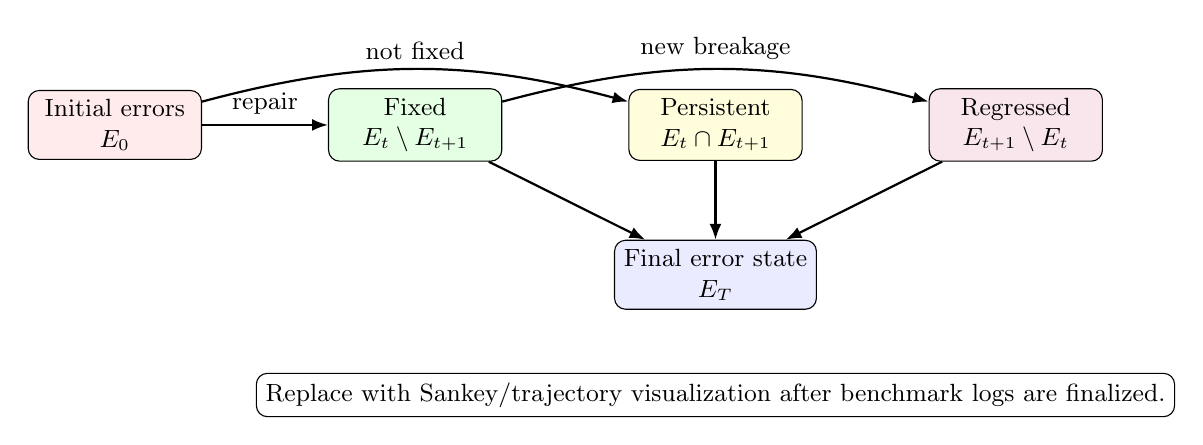
\begin{tikzpicture}[
    font=\small,
    state/.style={draw, rounded corners, align=center, minimum width=2.2cm, minimum height=0.85cm},
    arrow/.style={-{Latex[length=2mm]}, thick}
]
\node[state, fill=red!8] (err0) {Initial errors\\$E_0$};
\node[state, fill=green!10, right=16mm of err0] (fixed) {Fixed\\$E_t\setminus E_{t+1}$};
\node[state, fill=yellow!14, right=16mm of fixed] (persist) {Persistent\\$E_t\cap E_{t+1}$};
\node[state, fill=purple!10, right=16mm of persist] (regress) {Regressed\\$E_{t+1}\setminus E_t$};
\node[state, fill=blue!8, below=10mm of persist] (final) {Final error state\\$E_T$};

\draw[arrow] (err0) -- node[above] {repair} (fixed);
\draw[arrow] (err0) to[bend left=15] node[above] {not fixed} (persist);
\draw[arrow] (fixed) to[bend left=15] node[above] {new breakage} (regress);
\draw[arrow] (persist) -- (final);
\draw[arrow] (regress) -- (final);
\draw[arrow] (fixed) -- (final);

\node[draw, rounded corners, fill=white, align=center, below=8mm of final, minimum width=10cm]
{Replace with Sankey/trajectory visualization after benchmark logs are finalized.};
\end{tikzpicture}
\caption{Planned transition-flow visualization for fixed, persistent, and regressed error steps.}
\label{fig:sankey_placeholder}
\end{figure*}

\section{Failure Analysis Plan}
Failure analysis should be treated as a first-class part of the paper. Important categories include:
\begin{itemize}
    \item judges agreeing on an incorrect criticism,
    \item the prover satisfying flagged steps while weakening the theorem,
    \item corrections that increase proof length without improving rigor,
    \item assumptions added after the fact to rescue an invalid proof,
    \item high final verdicts despite unresolved mathematical uncertainty,
    \item repeated oscillation between two incompatible proof strategies.
\end{itemize}
For each category, the final paper should include one compact example with the original flagged step, the correction, the new evaluator response, and the resulting RACS transition.

\section{Limitations}
The proposed framework is not a substitute for formal verification. Its correctness is bounded by evaluator quality, prompt design, and the reliability of step-level error localization. JRS estimates relative reliability inside an ensemble but cannot certify mathematical truth. RACS measures correction transitions under a given evaluator signal; if the signal is wrong, the metric may reward an undesirable repair. Finally, the approach is designed for natural-language and LaTeX proofs, so adapting it to formal proof assistants would require a different error representation.

\section{Conclusion}
This paper presents a methodology for evaluating iterative LLM proof correction as a regression-aware trajectory problem. By combining step-level proof annotations, structured evaluator outputs, multi-judge reliability estimation, and RACS transition scoring, the framework exposes correction behaviors that final-verdict evaluation hides. The planned empirical sections will test how this framework behaves across OML proof tasks, baseline correction strategies, evaluator ensembles, and RACS weight configurations. The central claim to validate is not merely that iterative correction improves final proofs, but that correction dynamics can be measured, compared, and calibrated in a scientifically meaningful way.

\begin{thebibliography}{00}
\bibitem{lewkowycz2022minerva}
A. Lewkowycz, A. Andreassen, D. Dohan, E. Dyer, H. Michalewski, V. Ramasesh, A. Slone, C. Anil, I. Schlag, T. Gutman-Solo, Y. Wu, B. Neyshabur, G. Gur-Ari, and V. Misra, ``Solving Quantitative Reasoning Problems with Language Models,'' \emph{arXiv preprint arXiv:2206.14858}, 2022.

\bibitem{madaan2023selfrefine}
A. Madaan, N. Tandon, P. Clark, and Y. Yang, ``Self-Refine: Iterative Refinement with Self-Feedback,'' \emph{arXiv preprint arXiv:2303.17651}, 2023.

\bibitem{shinn2023reflexion}
N. Shinn, B. Labash, and A. Gopinath, ``Reflexion: Language Agents with Verbal Reinforcement Learning,'' \emph{Advances in Neural Information Processing Systems}, 2023.

\bibitem{zheng2023judging}
L. Zheng, W.-L. Chiang, Y. Sheng, S. Zhuang, Z. Wu, Y. Zhuang, Z. Lin, Z. Li, D. Li, E. Xing, H. Zhang, J. E. Gonzalez, and I. Stoica, ``Judging LLM-as-a-Judge with MT-Bench and Chatbot Arena,'' \emph{arXiv preprint arXiv:2306.05685}, 2023.

\bibitem{demoura2015lean}
L. de Moura, S. Kong, J. Avigad, F. van Doorn, and J. von Raumer, ``The Lean Theorem Prover,'' in \emph{International Conference on Automated Deduction}, 2015.
\end{thebibliography}

\end{document}
